\documentclass{report}

\usepackage[latin1]{inputenc}
\usepackage[T1]{fontenc}
\usepackage[francais]{babel}
\usepackage[top=2.5cm, bottom=2.5cm, left=2.5cm, right=2.5cm]{geometry}
\usepackage{graphicx}
\usepackage{amsmath,amsfonts,amssymb}
\usepackage{parallel}
\usepackage{float}
\restylefloat{table}

\usepackage[linesnumbered,algoruled,boxed,lined]{algorithm2e}

\setlength\parindent{24pt} % indentation paragraphes

\begin{document}
\begin{titlepage}

\newcommand{\HRule}{\rule{\linewidth}{0.5mm}} % Defines a new command for the horizontal lines, change thickness here

\center % Center everything on the page
 
%----------------------------------------------------------------------------------------
%	HEADING SECTIONS
%----------------------------------------------------------------------------------------

\textsc{\LARGE ENSEEIHT}\\[1.5cm] % Name of your university/college
\textsc{\Large Sémantique et TDL}\\[0.5cm] % Major heading such as course name
\textsc{\large Projet}\\[0.5cm] % Minor heading such as course title

%----------------------------------------------------------------------------------------
%	TITLE SECTION
%----------------------------------------------------------------------------------------

\HRule \\[0.4cm]
{ \huge \bfseries  Compilateur du langage $\mu$C^{\#}}\\[0.4cm] % Title of your document
\HRule \\[1.5cm]
 
%----------------------------------------------------------------------------------------
%	AUTHOR SECTION
%----------------------------------------------------------------------------------------

\emph{auteurs:}\\
\textsc{achard} - \textsc{vincent} \\
\textsc{barras} - \textsc{thomas} \\
\textsc{bouqsimi} - \textsc{amine} \\
\textsc{rigondaud} - \textsc{clément} \\

%----------------------------------------------------------------------------------------
%	DATE SECTION
%----------------------------------------------------------------------------------------

\date{} %enleve la date

%----------------------------------------------------------------------------------------
%	LOGO SECTION
%----------------------------------------------------------------------------------------

\vspace{7.2cm}
\begin{center}
%
\includegraphics[width=5]{N7.png}
\end{center}

%----------------------------------------------------------------------------------------

\vfill % Fill the rest of the page with whitespace

\end{titlepage}

\tableofcontents %table des matières.

\vfill

\chapter{Structure}

	\begin{figure}[H]
		\begin{center}
			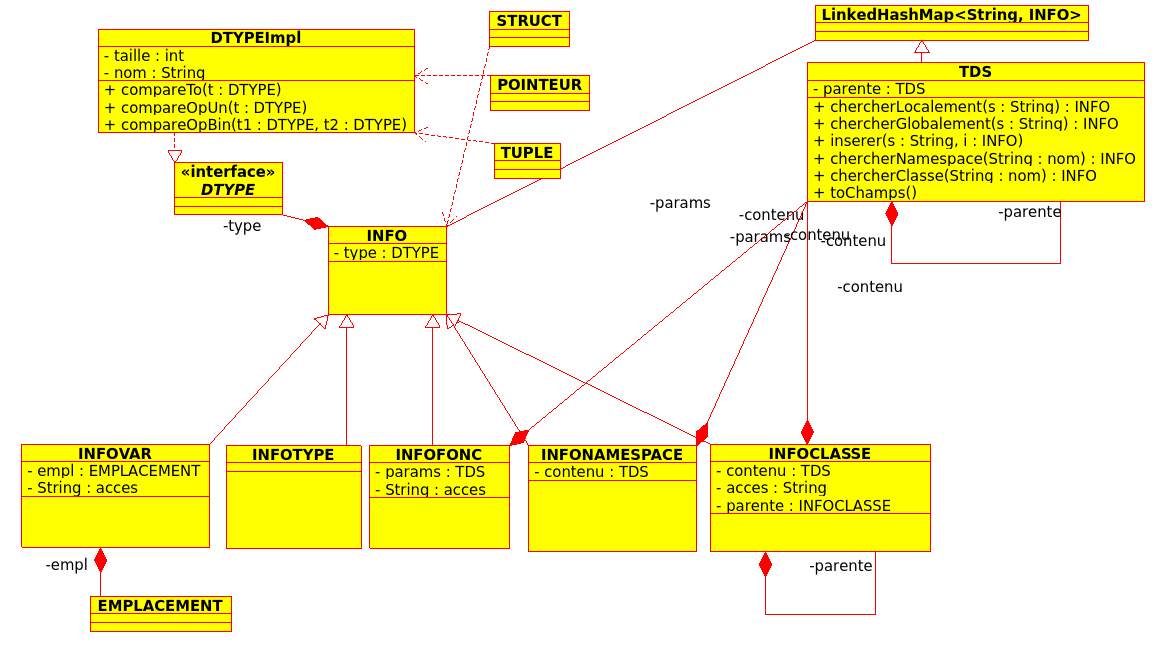
\includegraphics[scale=0.4]{UML.png}
		\end{center}
		\caption{UML global}
	\end{figure}
	
	\begin{figure}[H]
		\begin{center}
			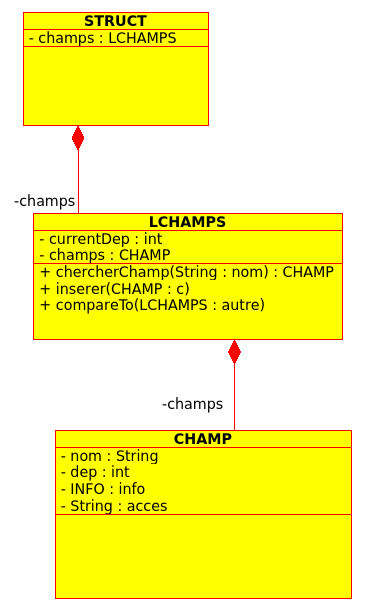
\includegraphics[scale=0.4]{UMLSTRUCT.png}
		\end{center}
		\caption{Précision STRUCT}
	\end{figure}

\chapter{Choix de conception}

\begin{itemize}
 
\end{itemize}

\chapter{Limitations}
\begin{itemize}

\end{itemize}



\end{document}